%%%%%%%%%%%%%%%%%%%%%%%%%%%%%%%%%%%%%%%%%%%%%%%%%%%%%%%%%%%%%%
% Universidade Federal do Pará
% Instututo de Tecnologia
% Faculdade de Engenharia da Computação e Telecomunicações
%
% Discente: Wederson Medeiros Silva
%
% Apresentação do Trabalho de Conclusão de Curso para
% obtenção do grau de Bacharel em Engenharia da Computação
% 
% Orientador: Prof. Dr. Roberto Menezes Rodrigues
% Co-orientador: Prof. Dr. Marco José de Sousa
%
%%%%%%%%%%%%%%%%%%%%%%%%%%%%%%%%%%%%%%%%%%%%%%%%%%%%%%%%%%%%%%

\documentclass{beamer}

% ---------------------------------------------------------------------------- %
% Para aceitar acentos e hifenização brasileira
% ---------------------------------------------------------------------------- %
\usepackage[brazil]{babel}
\usepackage[utf8]{inputenc}
% ---------------------------------------------------------------------------- %

% ---------------------------------------------------------------------------- %
% Características do tema escolhido
% ---------------------------------------------------------------------------- %
\usetheme{Hannover}
\usecolortheme{whale}
\usefonttheme{structurebold}
% ---------------------------------------------------------------------------- %

%\usepackage{graphicx}
\usepackage{graphics}
\graphicspath{ {figuras/} } 
%\usepackage[labelformat=empty]{caption}		% Para retirar todos os Fig. 1, Fig. 2, etc
%\setbeamertemplate{caption}[numbered]{}		% Para enumerar figuras
\usepackage[figurename=Fig.]{caption}

% Indice para cada seção (aparece antes de cada section) - TALVEZ EU USE
%\AtBeginSection[] {
%	\begin{frame}
%		\frametitle{\textbf{Agenda}}
%		\footnotesize{ \tableofcontents[currentsection,hideothersubsections] }
%	\end{frame}
%}

% ---------------------------------------------------------------------------- %
% Dados da apresentação
% ---------------------------------------------------------------------------- %
\logo{
\includegraphics[height=1.5cm]{logo_ufpa}}
\title[Carregador de baixo custo para baterias de Lítio]{Projeto de um carregador modular de baixo custo para baterias de íons de Lítio}
\author[Wederson Silva]{\textbf{Wederson Medeiros Silva} \\ \scriptsize{wederson.silva@itec.ufpa.br,\\ wederson18@gmail.com}} 
\institute[UFPA]{Universidade Federal do Pará \\  Instituto de Tecnologia \\ 
Faculdade de Engenharia da Computação e Telecomunicações}
\date{\today}

% ---------------------------------------------------------------------------- %

% ---------------------------------------------------------------------------- %
% Início do documento
% ---------------------------------------------------------------------------- %
\begin{document}

% ---------------------------------------------------------------------------- %
% Slide 0 (Capa???)
% ---------------------------------------------------------------------------- %
\begin{frame}
	\titlepage
\end{frame}
% ---------------------------------------------------------------------------- %

% ---------------------------------------------------------------------------- %
% Agenda da apresentação (Section especial)
% ---------------------------------------------------------------------------- %
\section*{Agenda}
	\begin{frame}
		\frametitle{Agenda}
		\tableofcontents[hidesubsections]
	\end{frame}
% ---------------------------------------------------------------------------- %

% ---------------------------------------------------------------------------- %
% Início da section - 
% ---------------------------------------------------------------------------- %
\section{Introdução}
	\subsection{Baterias de Lítio}	
	\begin{frame}\frametitle{Baterias de Lítio}		
	Usadas em diversos dispositivos...				\pause
	
	\begin{figure}[!ht]

	\begin{minipage}{\textwidth}
  \begin{minipage}{.45\textwidth}
      \centering
      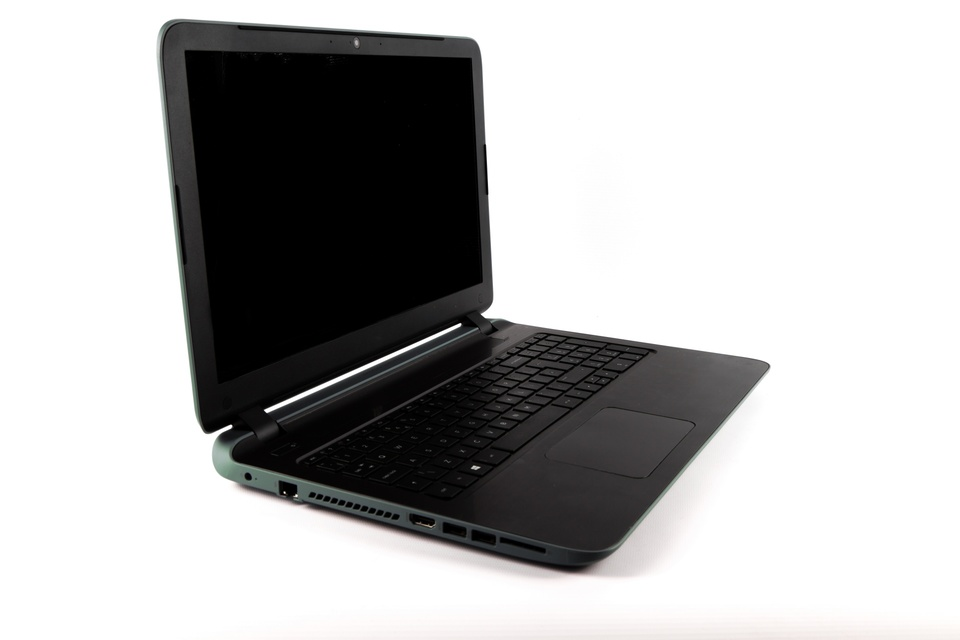
\includegraphics[width=.85\textwidth,scale=0.5]{laptop1}
      \caption{Notebook}
      \label{fig:laptop1}      
    \end{minipage}													\pause
%      Texto Qualquer
  \begin{minipage}{.45\textwidth}
    \center
      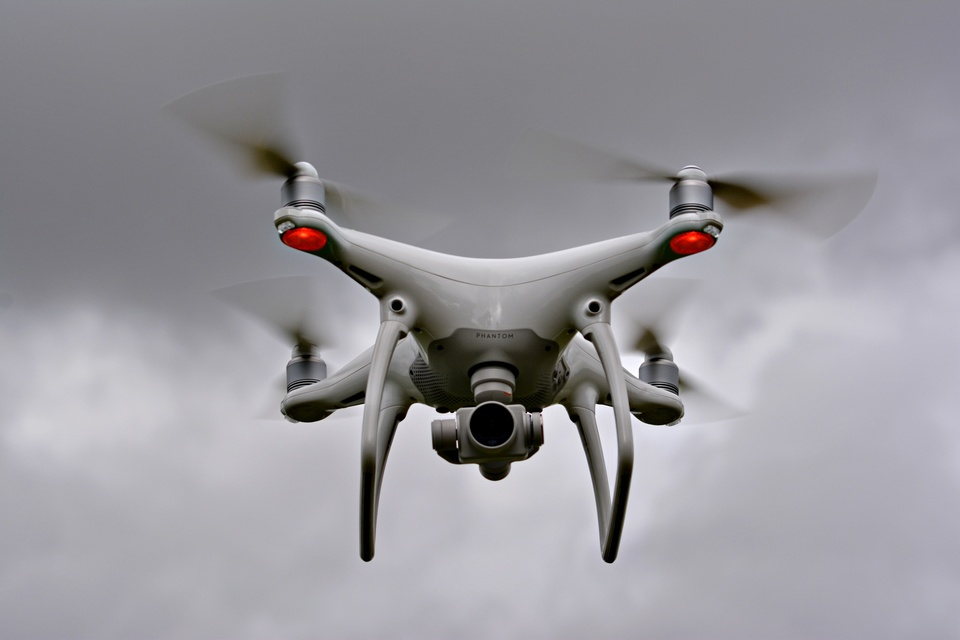
\includegraphics[width=.85\textwidth]{drone1}
      \caption{Drone}
      \label{fig:drone1}
    \end{minipage}
  \end{minipage}														\pause

	\begin{minipage}{\textwidth}
  \begin{minipage}{.45\textwidth}
      \centering
      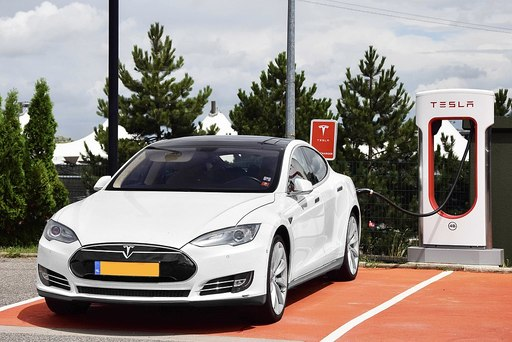
\includegraphics[width=.85\textwidth]{electric_car1}
      \caption{Carro elétrico}
			\label{fig:electric_car1}      
    \end{minipage}													\pause
  \begin{minipage}{.45\textwidth}
    \center
      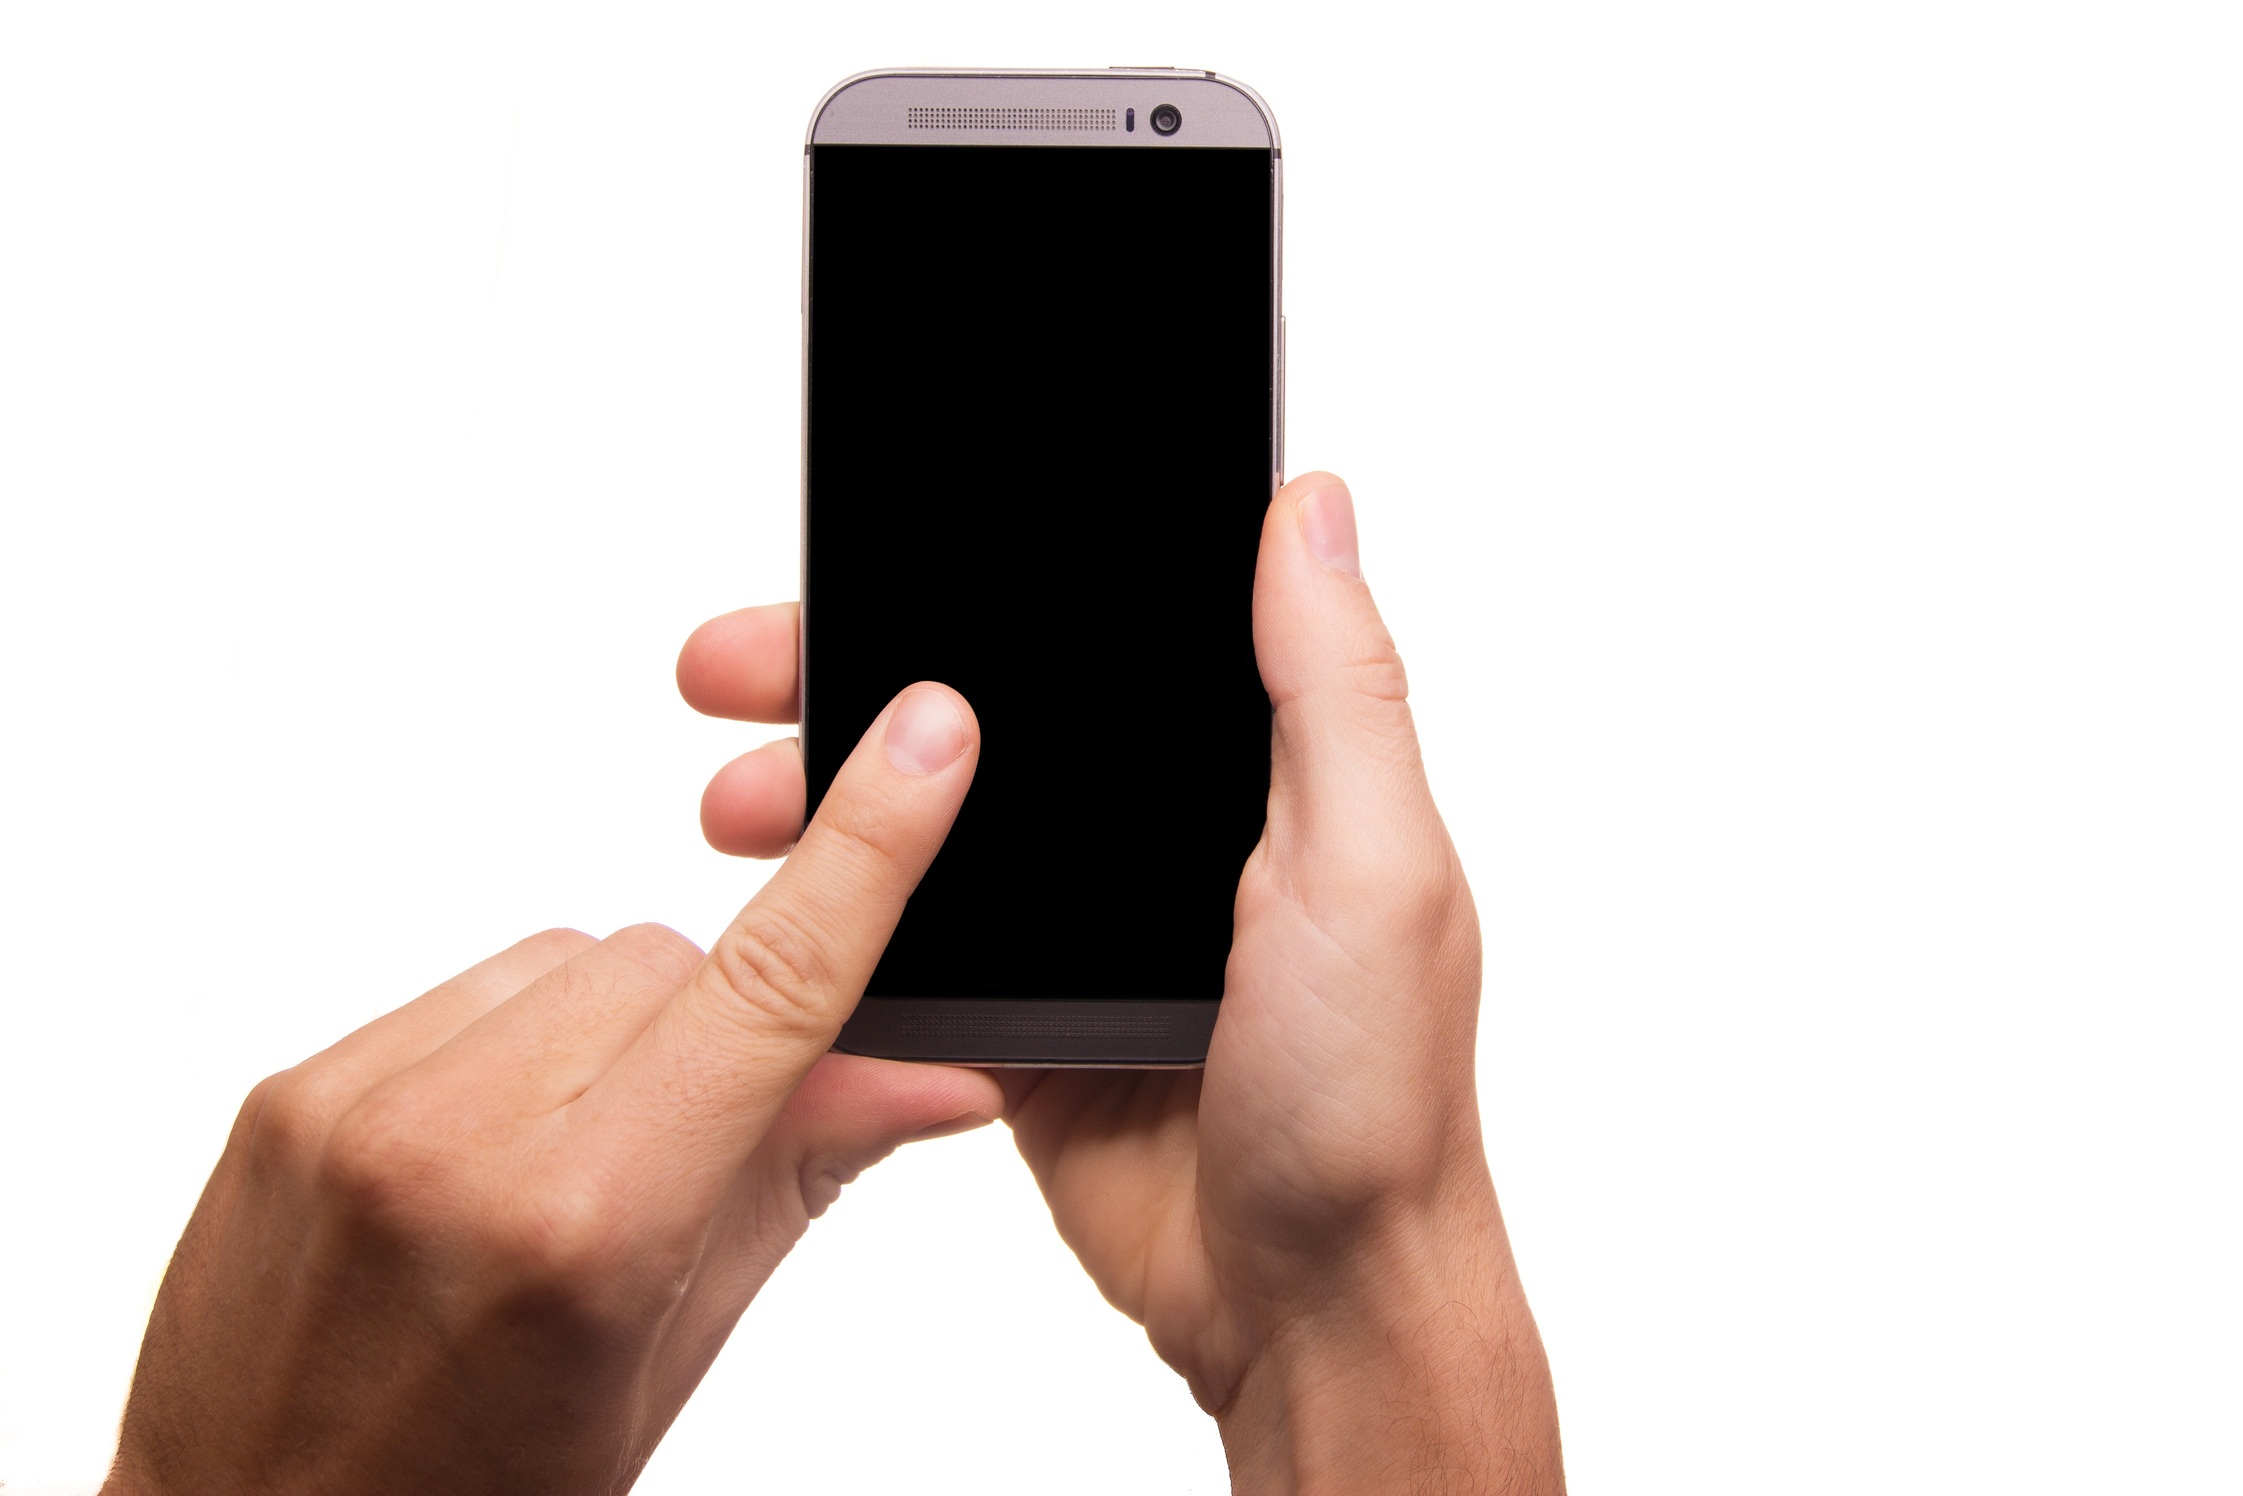
\includegraphics[width=.85\textwidth]{smartphone1}
      \caption{Smartphone}
      \label{fig:smartphone1}
    \end{minipage}
  \end{minipage}

	\end{figure}
\end{frame}		


\begin{frame}\frametitle{Baterias de Lítio}		
	Inclusive em brinquedos científicos...				\pause
	
\begin{figure}[h]
	\centering
	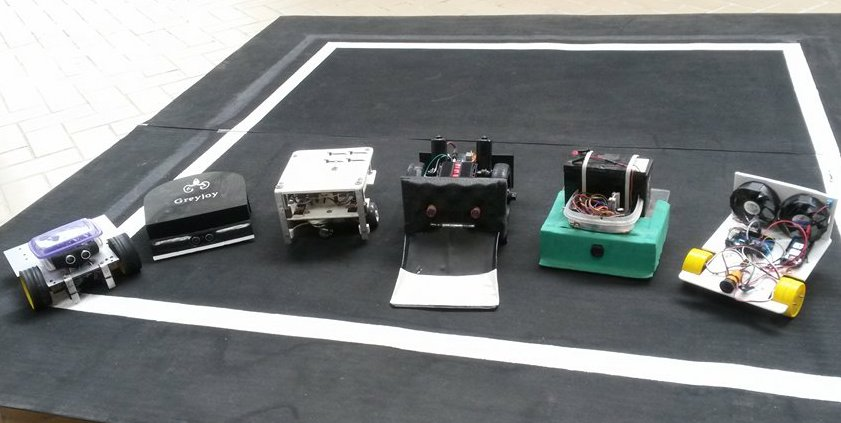
\includegraphics[width=\textwidth]{robos-sitec1}
	\caption{Robôs criados por diversos alunos}
	\label{fig:robos-sitec1}
\end{figure}
\end{frame}				
		
		
	\subsection{Carregadores}
	\begin{frame}\frametitle{Carregadores profissionais}
	Possuem preços elevados para projetos de baixo custo.
	
\begin{figure}[h]
	\centering
	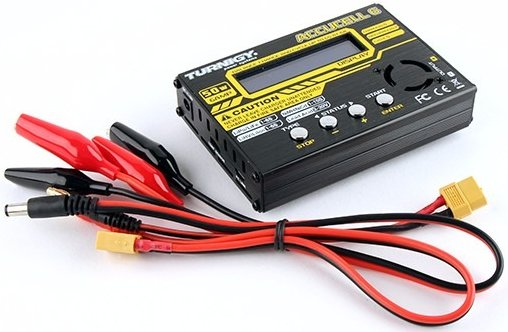
\includegraphics[width=0.85\textwidth]{charger1}
	\caption{Carregador profissional}
	\label{fig:charger1}
\end{figure}
\end{frame}							
	
	\subsection{Proposta de Solução}
	\begin{frame}\frametitle{Carregador proposto}
		
	\begin{columns}
	\column{.5\textwidth}	
			\centering
\alt<1>{\textcolor{green}{\textbf{{\huge \$\$\$\$\$\$\$\$\$\$}}}}{\textcolor{green}{\textbf{{\huge \$\$\$}}} \textbf{Baixo Custo}} 
	\begin{figure}[h]
		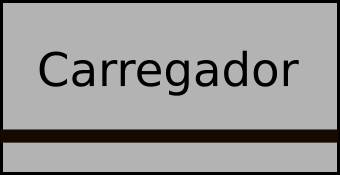
\includegraphics[width=.8\textwidth]{charger2}
%		\caption{Carregador profissional}
		\label{fig:charger2}		
	\end{figure}	\pause


	\column{.5\textwidth}
	\pause
			\centering				
			\textbf{Modular} 
		\begin{figure}[h]

		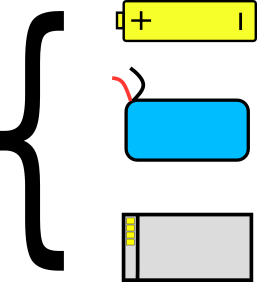
\includegraphics[width=.8\textwidth]{module1}
		\label{fig:module1}		
	\end{figure}		
	\end{columns}	\pause

			\centering				
			\textbf{Fácil Reprodução} 	
\begin{columns}
	\column{.25\textwidth}
	\begin{figure}[h]
		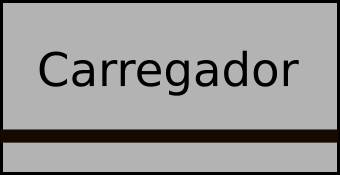
\includegraphics[width=\textwidth]{charger2}
	\end{figure}
	\column{.25\textwidth}
	\begin{figure}[h]
		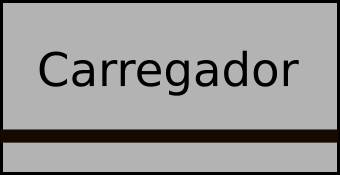
\includegraphics[width=\textwidth]{charger2}
	\end{figure}
	\column{.25\textwidth}
	\begin{figure}[h]
		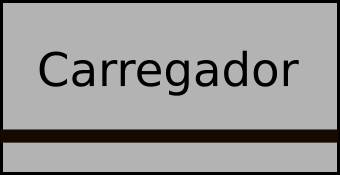
\includegraphics[width=\textwidth]{charger2}
	\end{figure}
	\column{.25\textwidth}
	\begin{figure}[h]
		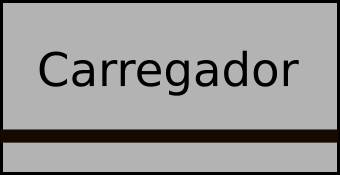
\includegraphics[width=\textwidth]{charger2}
	\end{figure}
\end{columns}	

	\end{frame}							
	

% ---------------------------------------------------------------------------- %

% ---------------------------------------------------------------------------- %
% Início da section - 
% ---------------------------------------------------------------------------- %
\section{Baterias de íons de Lítio}
	\subsection{Características}
		\begin{frame}\frametitle{Composição}
%	Escrever algo...
	
\begin{figure}[h]
	\centering
	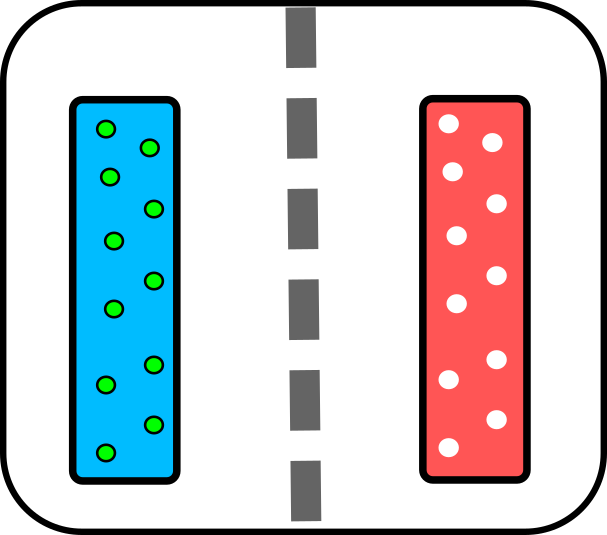
\includegraphics[width=0.70\textwidth]{battery-charged}
	\caption{Célula de Lítio carregada}
	\label{fig:battery-charged}
\end{figure}
\end{frame}							

\begin{frame}\frametitle{Composição}
%	Escrever algo...
	
\begin{figure}[h]
	\centering
	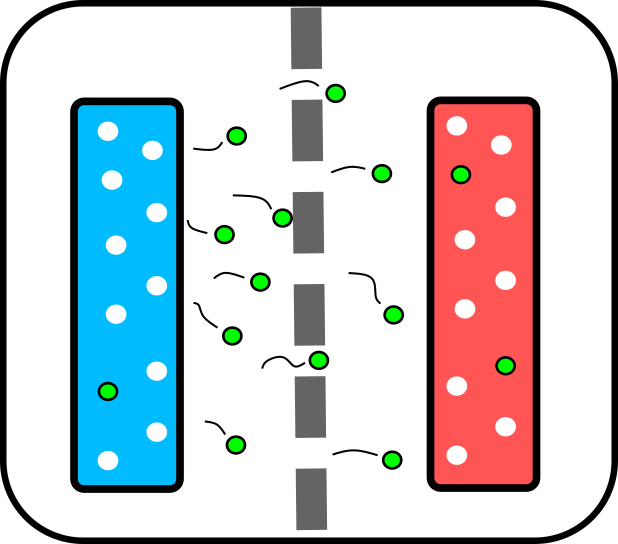
\includegraphics[width=0.70\textwidth]{battery-discharging}
	\caption{Célula de Lítio descarregando}
	\label{fig:battery-discharging}
\end{figure}
\end{frame}		

\begin{frame}\frametitle{Composição}
%	Escrever algo...
	
\begin{figure}[h]
	\centering
	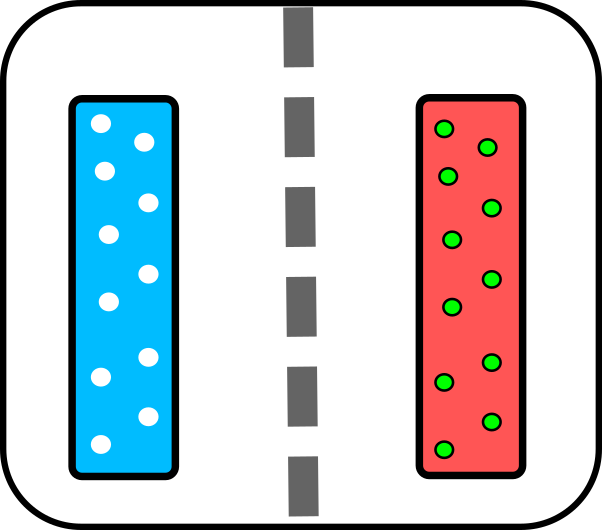
\includegraphics[width=0.70\textwidth]{battery-discharged}
	\caption{Célula de Lítio descarregada}
	\label{fig:battery-discharged}
\end{figure}
\end{frame}		

\begin{frame}\frametitle{Composição}
%	Escrever algo...
	
\begin{figure}[h]
	\centering
	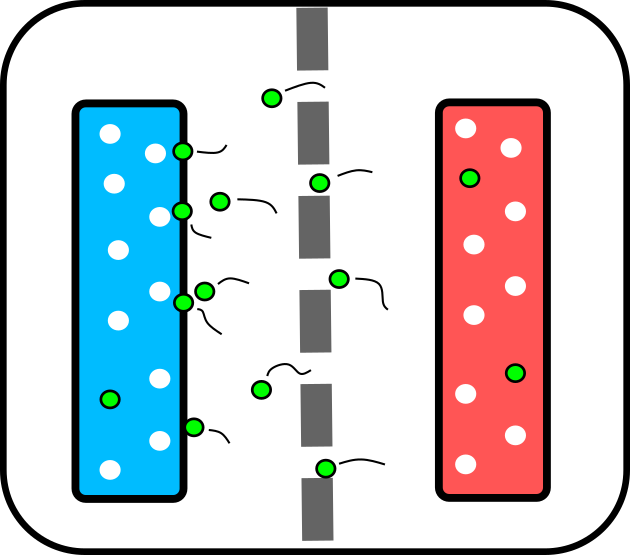
\includegraphics[width=0.70\textwidth]{battery-charging}
	\caption{Célula de Lítio carregando}
	\label{fig:battery-charging}
\end{figure}
\end{frame}				
	
	\subsection{Variações Químicas}
	\subsection{Formatos}
% ---------------------------------------------------------------------------- %
	
% ---------------------------------------------------------------------------- %
% Início da section - 
% ---------------------------------------------------------------------------- %
\section{Técnicas de carga}
	\subsection{Tradicional}
	\subsection{Técnica proposta}
% ---------------------------------------------------------------------------- %

% ---------------------------------------------------------------------------- %
% Início da section - 
% ---------------------------------------------------------------------------- %
\section{Circuitos e simulações}
	\subsection{Circuitos}
	\subsection{Simulações}
% ---------------------------------------------------------------------------- %

% ---------------------------------------------------------------------------- %
% Início da section - 
% ---------------------------------------------------------------------------- %
\section{Testes e Conclusões}
	\subsection{Testes}
	\subsection{Conclusões}
	\subsection{Trabalhos futuros}
% ---------------------------------------------------------------------------- %

\begin{frame}	% Isso força a criação da tabela
\end{frame} 	% de conteúdo completa

\end{document}
